\documentclass[11pt]{scrartcl}
\usepackage[sexy]{{style_files/evan}}

\usepackage{{style_files/NMC}}
\usepackage{standalone}
\usepackage{import}

\begin{document}
\title{NMC Problem Solutions \#1}
\date{Aug. 14, 2022} 
\maketitle

\section*{Welcome!}
    This document contains the solutions to the problems shown in the previous NMC problem set. We recommend not to check the solution to one particular problem unless you already tried it and ran out of ideas.\\
    We tried to make the solutions understandable and hope that you can see where each idea comes from. Keep in mind that the main idea of the problem is usually more important than the technical details.\\
    In any case, if you have trouble reading one (a passage is not clear, or you don't understand how someone could come up with one), just ask us!
    
\section{Algebra}

\textit{
    \begin{flushright}This is the field you're probably the most familiar with. It talks about\\
    \textbf{equations}, \textbf{inequalities}, \textbf{real} (and sometimes complex!) \textbf{numbers}, \textbf{polynomials}...\\
    despite your experience, these problems will require you to think\\
    in new ways not taught in class.\\
    Have fun and think creatively!\end{flushright}
}

\begin{enumerate}[label=\textbf{A\arabic*}.]
    \item Let's recall the associative law of addition: $a+(b+c) = (a+b)+c$, this allows us to reorder the parentheses in the equation:
    \[ 1 + \left(- \frac{1}{2} + \frac{1}{2}\right) + \left(- \frac{1}{3} + \frac{1}{3}\right) + \cdots + \left(-\frac{1}{99\,999}+\frac{1}{99\,999}\right) - \frac{1}{100\,000}. \]
    But now the value of the numbers in each pair of parentheses individually is $0$, so the expression equals $1+0+0+\cdots+0-1/100\,000 = 99\,999/100\,000$.
    
    \item Notice that a polynomial ``intersecting the $x$-axis" is equivalent to it having a real root. We will treat these two statements as synonymous in the proof.\\
    a) The polynomial $x^n + 1$ is an example of such a polynomial. Indeed, write $n=2m$ where $m$ is a integer, we find that if $x$ satisfies the equation $x^{2m} + 1 = 0$, then $y=x^m$ must satisfy $y^2 + 1 = 0$, which we already know has no solution as the text described.\\
    b) The general idea is to zoom out the graph of a polynomial: you might notice a pattern. It looks like for odd-degree polynomials (whose leading coefficient is positive), if you pick a very negative number, the graph will be below the $x$-axis, while if you pick a very positive number, the graph will be above the $x$-axis. But the graph is continuous (meaning it has no jumps or cuts, it can be drawn with a pen without lifting it from the paper), so if there are two points, one above and one below the line, since they're connected together by the graph, the graph must cross the line at some point.\\
    But how do we know these very negative/positive points exist? Pick a positive integer $n$, it is sufficient to prove that for all positive constants $c$ and polynomials $p(x)$ of degree less than $n$, there exists an $Y>0$ such that for all $x$ such that for all $|x| > Y$, we have that $|cx^n| > |p(x)|$. After all, our polynomial of degree $n$ can then be written in the form $cx^n + p(x)$, or $-(cx^n + p(x))$ if the coefficient of the $x^n$ is negative.\\
    So indeed, suppose $p(x) = a_{n-1}x^{n-1} + \cdots + a_0$, then $|p(x)| < (|a_{n-1}| + \cdots + |a_0|)|x^{n-1}| = A|x^{n-1}|$ for all $x>1$, so it suffices to show there's some $Y>1$ such that for all $x$ with $|x|>Y$: $$|cx^n| > A|x^{n-1}| \Longleftrightarrow |cx| > A.$$
    But then in fact any $Y\ge A/c$ works. So that means that we eventually do always stay `very' positive (if we have a positive $x^n$-coefficient) or negative (if we have a negative $x^n$-coefficient) in the long run.
\end{enumerate}

\newpage
\section{Combinatorics}
\textit{\begin{flushright}
Combinatorics is a branch of mathematics that primarily deals with\\
\textbf{counting} things in efficient ways, but here we also include \textbf{games}\\
and other creative problems that don't fit in the other categories.\\
Enjoy this playful chapter!
\end{flushright}}

\begin{enumerate}[label=\textbf{C\arabic*}.]
    \item There are two ways to solve this problem, one uses the technique of infinite series, and the other is a clever variable trick.\\
    \textbf{Solution 1: a clever variable trick.} We'll first find the probability $p$ that Frog wins, then the probability that Arky wins will be $100\%-p$. Let's consider the ways Frog could win: he could toss heads with $1/2$ probability, in that case he wins immediately, otherwise there's a $1/2$ chance that he doesn't win and the coin is handed to Arky, then Frog has to hope that Arky gets the $1/2$ chance that they don't win and the coin is handed back to him, but notice, now we're in the same situation as before, so the probability that Frog wins, given that Frog and Arky both lose on their own first round is the original probability again. In other words:
    \begin{align*}
    p &= \frac{1}{2} + \frac{1}{2} \cdot \frac{1}{2} \cdot p\\
    \Leftrightarrow p &= \frac{2}{3}.
    \end{align*}
    And so Arky has a $1-p = \boxed{1/3}$, or $33.3\%$ chance of winning.\\
    a) We can reason in the same way as above, but this time the equation is $p = 1/6 + 5/6 \cdot 5/6 \cdot p$, which implies $p = 6/11$ and so Arky has a $1-p=\boxed{5/11}$ chance of winning.\\
    b) Let $q$ be the probability that $P_n$ wins, he could either hope that the first $n-1$ players lose and then win immediately on his own turn which has a chance of $1/2^n$ of happening, or otherwise all the players lose in their first round, which also has a chance of $1/2^n$ of happening, but in this last case we're back at the starting position, so we get the equation:
    \begin{align*}
    q &= \frac{1}{2^n} + \frac{1}{2^n}q\\
    \Leftrightarrow q &= \boxed{\frac{1}{2^n-1}}.
    \end{align*}
    In the case we're using dices, the equation is $q = (5/6)^{n-1}\cdot 1/6 + (5/6)^n q \Leftrightarrow q = 5^{n-1}/(6^n-1)$.\\
    \textbf{Solution 2: infinite series.}
    Let's list all possible ways Arky could win:
    \begin{itemize}
        \item Frog loses; Arky wins.
        \item Frog loses; Arky loses; Frog loses; Arky wins.
        \item Frog loses; Arky loses; Frog loses; Arky loses; Frog loses; Arky wins.
        \item $\cdots$.
    \end{itemize}
    The first scenario has chance $1/4$ of happening, the second $1/4^2$, the third $1/4^3$ and so on... so the probability that Arky wins must be described by this infinite sum:
    $$S = 1/4 + 1/4^2 + 1/4^3 + \cdots.$$
    How does one even calculate an infinite sum? What does it mean? The trick is to look at \textit{partial} sums: finite segments of the sum.
    $$S_n = \underbrace{1/4 + 1/4^2 + \cdots + 1/4^n}_\text{Finite, as it only contains $n$ terms}$$
    There's something really nice about this series, look at what happens when we multiply it by $3$ and add $1/4^n$:
    \begin{align*}
        3S_n + \frac1{4^n} &= \frac34 + \cdots \frac3{4^{n-2}} + \frac3{4^{n-1}} + \mathbf{\frac3{4^n} + \frac{1}{4^n}}\\
        &= \frac34 + \cdots \frac3{4^{n-2}} + \frac3{4^{n-1}} + \mathbf{\frac4{4^n}}\\
        &= \frac34 + \cdots \frac3{4^{n-2}} + \mathbf{\frac3{4^{n-1}} + \frac1{4^{n-1}}}\\
        &= \frac34 + \cdots \frac3{4^{n-2}} + \mathbf{\frac4{4^{n-1}}} \\
        &= \frac34 + \cdots \mathbf{\frac3{4^{n-2}} + \frac1{4^{n-2}}} \\
        &\cdots\\
        3S_n + \frac1{4^n} &= \frac{3}{4} + \frac{1}{4} = 1\\
        \Leftrightarrow S_n &= \frac{1-1/4^n}{3}
    \end{align*}
    This allows us to write $S_n$ in a very compact form! But what for? Well, once we can write something compactly, we can ask what happens as we increase the value of $n$ larger and larger: the limit that $S_n$ approaches should then be equal to $S$, the sum of all infinite terms. In this case, as $n$ increases, $1/4^n$ becomes smaller and smaller and eventually $0$, while the other terms remain constant, and so the result os $(1-0)/3 = \boxed{1/3}$, or $33.3\%$.\\
    a) We calculate the following infinite series:
    \begin{align*}
    &\frac56 \cdot \frac16 + \left(\frac56\right)^3 \cdot \frac16 + \left(\frac56\right)^5 \cdot \frac16 + \cdots\\
    =&\frac56\cdot\frac16\cdot\left(1 + \frac{25}{36} + \left(\frac{25}{36}\right)^2 + \cdots\right)\\
    =&\frac56\cdot\frac16\cdot\frac{36}{11} = \boxed{\frac{5}{11}}.
    \end{align*}
    b) For a similar reason to solution $1$ the series is:
    $$\frac{1}{2^n} + \frac{1}{(2^n)^2} + \frac{1}{(2^n)^3} + \cdots = \boxed{\frac{1}{2^n-1}}$$
    % hi hehe <33333
    % :nikoblush: <3333333

    \item Note that Niko is bringing a given sequence back to an `unjumbled' state with every move: there keep being more lightbulbs of the same type together. To formalize this, we look at the number of `chains' of lightbulbs together, since we are done unjumbling if we get just $2$ chains. As an example, let's look at how the sequence $ABAABAABBB$ gets un-jumbled by Niko.
    
    \begin{table}[ht]
    \centering
    \begin{tabular}{l|l}
    \textbf{Sequence} & \textbf{Number of chains} \\ \hline
    $ABAABAABBB$ & 6 \\
    $BABAAAABBB$ & 5 \\
    $AAAABABBBB$ & 4 \\
    $BAAAAABBBB$ & 3 \\
    $AAAAABBBBB$ & 2 \\
    $AAAAABBBBB$ & 2 \\
    $\cdots$     & $\cdots$
    \end{tabular}
    \end{table}
    
    \vspace{2cm}
    
    The number of chains decreases by $1$ every step that it is not $2$! And we can see why this is true: if the first $n$ lightbulbs aren't all of the same type, then the $n$\textsuperscript{th} lightbulb won't be contained by the leftmost chain, and neither the rightmost chain (since all chains are at most $n$ bulbs anyway). So that means we are putting a chain in the middle at the beginning. This means that the two surrounding chains merge into one, and so the number of chains decreases by exactly $1$.
    
    And since the number of chains is finite, Niko will always reduce the number of chains to $2$ after some number of moves, at which point we indeed have that the first $n$ lightbulbs are all of the same type.
    
    \emph{Note: a generalization (\fullchili \fullchili) actually appeared on the International Mathematical Olympiad of 2022! Let Niko pick the maximal group containing the $k$\textsuperscript{th} lightbulb each time for some $1 \le k \le 2n$: then for what pairs $(n,k)$ can Niko always unjumble the sequence?} 
    \end{enumerate}
    

\newpage
\section{Geometry}
\textit{\begin{flushright}
Geometry, studied since ancient Greece, is the oldest discipline of mathematics. It concerns \textbf{space}, \textbf{distances}, \textbf{areas}, \textbf{volumes}.\\ Learn the pretty intricacies of the figures below!
\end{flushright}}

\begin{enumerate}[label=\textbf{G\arabic*}.]
    \item %Below is a triangle $ABC$ whose area is $60$. $M$ and $N$ cut segments $BC$ and $AC$ in half respectively, what's the value of the blue area $[ABM]$? What about the orange $[CMN]$ or green one $[MGN]$?

    Surprisingly, all we need for this problem is the following fact: the area of a triangle is half of the product of a base times the corresponding height.
    
    \begin{figure}[h]
        \centering
        \includegraphics[width=5cm]{Diagrams/G1.tex}
        \label{fig:NMC1_G1}
    \end{figure}
    
    Let's see how we can apply it to the blue area $[ABM]$ if we pick $BM$ as its base: it has a base $BM$ that is half the length of the original triangle's $BC$, but has the same height (since $BM$ and $BC$ are the same line). This means that $[ABM] = [ABC]/2 = \boxed{30}$, or in an equation:
    \[
      [ABM] = BM \cdot d(A,BM) /2 = (BC/2) \cdot d(BC) /2 = [ABC]/2 = \boxed{30}. 
    \]
    Here, $d(X,YZ)$ denotes the (perpendicular) distance from point $X$ to line $YZ$, a more formal definition of `height'.
    
    For the orange triangle $\triangle ABC$, we can already see that it looks `similar' to $\triangle NMC$. And in fact it does: since $CA/CN = 2 = CB/CM$ we know that $\triangle ABC \sim \triangle NMC$ with scaling factor $2$, so $[NMC] = \frac{1}{2^2} [ABC] = \boxed{15}$. However, a bit more intuitively we can also say that a \emph{homothety} from $C$ sends $\triangle ABC$ to $\triangle NMC$ by multiplying $A$ and $B$ with respect to $C$ with a factor $\frac12$ to get $N$ and $M$. This leads to the same thing.
    
    So now we know that $AB = 2MN$ and furthermore $AB \parallel MN$ (all by $\triangle ABC \sim \triangle NMC$). So we again have the homothety $\triangle GAB \sim \triangle GMN$ with a factor of $-\frac12$ this time, so if we take $MN = AB/2$ to be the base of $\triangle GMN$ then its height is $1/3$ of the distance between $AB$ and $MN$, and that distance itself is half of $d(C, AB)$ by our first homothety. So \[ [GMN] = \frac12 \cdot \frac13 \cdot \frac 12 [ABC] = \frac12 [ABC] = \boxed{5}. \]
    
    \item 
    
    \begin{figure}[h]
        \centering
        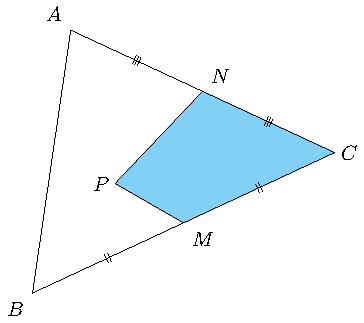
\includegraphics[width=6cm, page=1]{Diagrams/G2sol.pdf}
        \includegraphics[width=6cm, page=4]{Diagrams/G2sol.pdf}
    \end{figure}
    
    Since $CA/CN = 2 = CB/CM$, we know that the line $MN$ is actually parallel to $AB$. This is convenient because the area of the quadrilateral $PMCN$ can be divided into two triangles: $\triangle PMN$ and $\triangle MNC$, the area of $\triangle MNC$. We already calculated the latter in the previous question and shown it's $15$, and this already tells us that the quadrilateral $PMCN$ has area at least $15$. Furthermore, the area of triangle $PMN$ depends only on the height of $P$ on $MN$, since the base is fixed. The highest $P$ can be is in fact on any point of line $AB$, for example on $A$, but on that point we can check that the quadrilateral actually becomes the triangle $\triangle AMC$, because the sides $NP$ and $NC$ flatten into one. We know that area is half the triangle, which is $30$, so the area of $PMCN$ is at most $30$, and that finishes the proof.

    \begin{figure}[h]
        \centering
        \includegraphics[width=6cm, page=3]{Diagrams/G2sol.pdf}
    \end{figure}

    \item \begin{enumerate}[label=(\alph*)]
        \item %Let $ABCD$ be a quadrilateral. Show that if two opposite angles of $ABCD$ are both right angles, then there is a circle that passes through the vertices of the quadrilateral.

We turn to Thales's theorem: if $\triangle BAD$ is a right triangle with $\angle BAD = 90^\circ$ then its  circumcenter (the center of the circle passing through all three vertices of the triangle) is the midpoint $M$ of the hypotenuse $BD$. We can prove this as follows:
        
        \begin{center}
        \begin{tikzpicture}[scale=2.4]
  \draw[dotted] (0,0) circle (1);

  \foreach \point [count = \n, evaluate = \n as \rot using {{100,140,200,320,280}[\n - 1]}] in {A,B,C,D,A'}{
    \coordinate (\point) at (\rot:1);
    %\fill (\point) circle (1pt);
    \node[label={[label distance=-7pt]\rot:$\point$}] at (\point) {};
  }

  \draw (A) -- (B) -- (C) -- (D) -- cycle;
  \tkzMarkRightAngles[size=0.12](B,A,D D,C,B)

  \draw (B) -- (D);
  \tkzDefMidPoint(B,D) \tkzGetPoint{M}
  \node[label={[label distance=-7pt]15:$M$}] at (M) {};

  \draw (M) -- (A) (M) -- (C);
  
  \tkzDrawSegments[dotted](M,A' D,A' B,A' A',D)
  \tkzMarkSegments[pos=.5,mark=|](M,A M,B M,C M,D M,A')
\end{tikzpicture}
\end{center}
        
        Let $A'$ be the reflection of $A$ in $M$. Then $BADA'$ is a parallelogram (since we have two diagonals crossing in their midpoint). But since $\angle BAD = 90^\circ$ we must even have a rectangle. In a rectangle, the diagonals have an equal length: so $|MA| = |MB| = |MD|$, which means that $M$ is the circumcenter of $\triangle BAD$.
        
        Similarly, $M$ is also the circumcenter of $\triangle BCD$. So $M$ is the center of the circle passing through all four points $A, B, C, D$ at once, which is what we wanted to find.
        
        \item %Let $ABCD$ be a quadrilateral. Show that if two opposite angles of $ABCD$ are supplementary (that means they sum to $180^\circ$), then there is a circle that passes through the vertices of the quadrilateral.
        %
        We first note the (important!) converse: if we have a cyclic quadrilateral (a quadrilateral for which there exists a circle that passes through all $4$ vertices) then opposite angles are supplementary. We can see this by introducing the circumcenter and then proving that the sum of two opposite angles is equal to the sum of the two other opposite angles. And since the sum of all angles in a (general) quadrilateral is $360^\circ$, we know that the single sum of two opposite angle is always $180^\circ$.
        
        Let $\Gamma$ be the circumcircle (the circle passing through all three vertices of a triangle) of $\triangle BCD$. We want to prove that $A$ also lies on $\Gamma$. Suppose it did not. Then we have two cases: either $A$ lies outside of $\Gamma$ or inside. We also note that since $\angle A + \angle C = \angle B + \angle D = 180^\circ$, all internal angles of the quadrilateral are less than $180^\circ$, so $A$ and $C$ are on different sides of $BD$.
        
        \begin{center}
        \begin{tikzpicture}[scale=2.3]
  \draw[dotted] (0,0) circle (1);

  \foreach \point [count = \n, evaluate = \n as \rot using {{190,240,20}[\n - 1]}] in {B,C,D}{
    \coordinate (\point) at (\rot:1);
    %\fill (\point) circle (1pt);
    \node[label={[label distance=-7pt]\rot:$\point$}] at (\point) {};
  }

  \coordinate (A) at (120:1.3);
  \node[label={[label distance=-7pt]120:$A$}] at (A) {};

  \draw (A) -- (B) -- (C) -- (D) -- cycle;

  \tkzMarkAngle[mark=|,size=0.12cm](B,A,D)
  \tkzMarkAngle[mark=||,size=0.12cm](D,C,B)
\end{tikzpicture}
        \begin{tikzpicture}[scale=2.3]
  \draw[dotted] (0,0) circle (1);

  \foreach \point [count = \n, evaluate = \n as \rot using {{190,240,20}[\n - 1]}] in {B,C,D}{
    \coordinate (\point) at (\rot:1);
    %\fill (\point) circle (1pt);
    \node[label={[label distance=-7pt]\rot:$\point$}] at (\point) {};
  }

  \coordinate (A) at (120:0.7);
  \node[label={[label distance=-7pt]120:$A$}] at (A) {};

  \draw (A) -- (B) -- (C) -- (D) -- cycle;

  \tkzMarkAngle[mark=|,size=0.12cm](B,A,D)
  \tkzMarkAngle[mark=||,size=0.12cm](D,C,B)
\end{tikzpicture}
        \end{center}
        
        Now intersect the line $CA$ with $\Gamma$ in another point $A' \ne C$, such that we do get a cyclic quadrilateral $A'BCD$.
        
        \begin{center}
            \begin{tikzpicture}[scale=2.3]
  \coordinate (O) at (0,0);
  \draw[dotted] (0,0) circle (1);

  \foreach \point [count = \n, evaluate = \n as \rot using {{190,240,20}[\n - 1]}] in {B,C,D}{
    \coordinate (\point) at (\rot:1);
    %\fill (\point) circle (1pt);
    \node[label={[label distance=-7pt]\rot:$\point$}] at (\point) {};
  }

  \coordinate (A) at (120:1.3);
  \node[label={[label distance=-7pt]120:$A$}] at (A) {};

  \draw (A) -- (B) -- (C) -- (D) -- cycle;

  \tkzMarkAngle[mark=|,size=0.12cm](B,A,D)
  \tkzMarkAngle[mark=||,size=0.12cm](D,C,B)

  \tkzInterLC(C,A)(O,C) \tkzGetPoints{A'}{A''};
  \node[label={[label distance=-7pt]50:$A'$}] at (A') {};
  \draw (B) -- (A') -- (D);

  \draw (C) -- (A);
  \draw (B) -- (D);

  \tkzMarkAngle[mark=|,size=0.12cm](B,A',D)
\end{tikzpicture}
            \begin{tikzpicture}[scale=2.3]
  \coordinate (O) at (0,0);
  \draw[dotted] (0,0) circle (1);

  \foreach \point [count = \n, evaluate = \n as \rot using {{190,240,20}[\n - 1]}] in {B,C,D}{
    \coordinate (\point) at (\rot:1);
    %\fill (\point) circle (1pt);
    \node[label={[label distance=-7pt]\rot:$\point$}] at (\point) {};
  }

  \coordinate (A) at (120:0.7);
  \node[label={[label distance=-7pt]10:$A$}] at (A) {};

  \draw (A) -- (B) -- (C) -- (D) -- cycle;

  \tkzMarkAngle[mark=|,size=0.12cm](B,A,D)
  \tkzMarkAngle[mark=||,size=0.12cm](D,C,B)

  \tkzInterLC(C,A)(O,C) \tkzGetPoints{A'}{A''};;
  \node[label={[label distance=-5pt]90:$A'$}] at (A') {};
  \draw (B) -- (A') -- (D);

  \draw (C) -- (A');
  \draw (B) -- (D);

  \tkzMarkAngle[mark=|,size=0.12cm](B,A',D)
\end{tikzpicture}
        \end{center}
        
        Now note that both $\angle BAD$ and $\angle BA'D$ are supplementary to $\angle BCD$, so $\angle BAD = \angle BA'D$.
        
        But now note that $\angle ABD + \angle BDA$ is supplementary to $\angle BAD$, just like $\angle A'BD + \angle BDA'$ is supplementary to $\angle BA'D$. But since $\angle BAD = \angle BA'D$, we must have $\angle ABD + \angle BDA = \angle A'BD + \angle BDA'$. But this gives problems: if $A$ lies outside of $\Gamma$ then $\angle ABD > \angle A'BD$ and $\angle BDA > \angle BDA'$ so actually $\angle ABD + \angle BDA > \angle A'BD + \angle BDA'$, and if $A$ lies inside of $\Gamma$ we flip the signs. So $A$ cannot lie either outside or inside of $\Gamma$: it has to lie exactly on $\Gamma$.
        
        \emph{You could also intersect the line $AB$ with $\Gamma$, in which case you would get that $\angle BA'D = \angle BAD$ so $A'D \parallel AD$ so $A = A'$!}
    \end{enumerate}
    
%    \begin{figure}[h]
%        \centering
%        \includegraphics[width=10cm]{Diagrams/G2.tex}
%        \label{fig:NMC1_G2}
%    \end{figure}
    
    %\item In a triangle $ABC$, we let the lengths of sides $BC, CA, AB$ be denoted by $a, b, c$ respectively (so the letter refers to the side across it), and the angles at $A, B, C$ be denoted by $\alpha, \beta, \gamma$ respectively.
    %\begin{enumerate}[label=(\alph*)]
    %    \item Suppose $\alpha = 90^\circ$. Prove that the hypotenuse $BC$ is the greatest side, so $a > b$ and $a > c$.
    %    \item Suppose $\alpha > 90^\circ$. Prove that $BC$ is the greatest side.
    %    \item Suppose $\alpha > \beta > \gamma$. Does it always hold that $a > b > c$? What about the converse (if $a > b > c$ then $\alpha > \beta > \gamma$)?
    %\end{enumerate}
\end{enumerate}

\newpage
\section{Number Theory}
\textit{\begin{flushright}
Number theory is the part of mathematics that deals with the\\ \textbf{integers} (numbers w/ no decimal dot), \textbf{factorization}, \textbf{divisibility}, \textbf{primes}, ...\\ While its objects are simple, don't be deceived,\\ solutions still require a good bit of cleverness!
\end{flushright}}
\begin{enumerate}[label=\textbf{N\arabic*}.]
    \item \textbf{Part $1$: $2^{2022}$}. Instead of calculating the whole number $2^{2022}$ at once, we take a look at the last digit of the smaller values of $2^n$. Here's a table listing the first $8$:
    
    \begin{table}[ht]
    \centering
    \begin{tabular}{c|r}
    \textbf{$n$} & \textbf{$2^n$} \\ 
    \hline
    $1$ & $\color{cyan}2$ \\
    $2$ & $\color{cyan}4$ \\
    $3$ & $\color{cyan}8$ \\
    $4$ & $1\color{cyan}6$ \\
    $5$ & $3\color{cyan}2$ \\
    $5$ & $6\color{cyan}4$ \\
    $6$ & $12\color{cyan}8$ \\
    $7$ & $25\color{cyan}6$ \\
    $8$ & $51\color{cyan}2$ \\
    $\cdots$ & $\cdots$
    \end{tabular}
    \end{table}
    
    It looks like the units digit follow a cyclic pattern that repeats every $4$ numbers: $2,4,8,6,(repeat)$. Why is that? Think about what happens when you multiply two numbers together using long multiplication:
    
    \begin{table}[ht]
    \centering
    \begin{tabular}{ccccc}
    &  &   & $2$ & $\times$\\
    &$5$ & $1$ & $2$ & $=$ \\
    \hline
    &  &   & \color{red}$4$\\
    &  & 2 & \color{red}$0$\\
    $1$ & $0$ & $0$ & \color{red}$0$\\
      \hline
    $1$ & $0$ & $2$ & \color{red}$4$ 
    \end{tabular}
    \end{table}
    
    Long multiplication is done in two parts: you first multiply the top number by every digit of the bottom number, then place them with the right off-set and sum all the results. But in the summing part, all but the first result end with a $0$, this is because they're off-set according to the position of the original digit. But what this means is that \textbf{to tell what the last digit of a product of two numbers is, you only need to care about the last digits of those two numbers!} All other digits cannot change the result.\\
    So in particular, since $2^5$ ends with a $2$, the pattern of the last digit must repeat from that point onward, because all digits other than the last one don't matter. Now according to our pattern, for any number $n$ that is exactly $2$ above a multiple of $4$, $2^n$ ends with $4$, so since $2022 = 2020 + 2 = 505\times4+2$, we know that $2^{2022}$ ends with the digit $\boxed{4}$.\\
    \textbf{Part $2$: $2^{2^{2022}}$.} Recall the pattern that we discovered in part $1$: according to it, if $n$ is a multiple of $4$, then $2^n$ ends with the digit $6$. Now clearly $2^{2022}$ is a multiple of $4 = 2\times 2$, so the last digit of $2^{2^{2022}}$ is $\boxed{6}$.\\
    \textbf{Part $3$: $3^{2006}/5$.} The remainders of numbers when they're divided by $5$ have a strong connection to their last digit, so if we can tell what the last digit of $3^{2006}$ is we're done. We can try the same idea as before, form a sequence of last digits until you notice it repeats: $3^1 = \color{orange}3$, $3^2 = 9$, $3^3 = 27$, $3^4 = 81$, $3^5 = 24\color{orange}3$. Again it looks like this sequence repeats every $4$ numbers. $2006 = 2004 + 2 = 501\times 4 + 2$, so $3^{2006}$ ends with the digit $9$, which implies that when it's divided by $5$, the residue is $\boxed{4}$.
    \textbf{Part $4$: $3^{2006}/8$.} Sadly, divisibility by $8$ is not strongly connected to the last digit of a number. For example $2$ leaves remainder $2$ when divided by $8$, but $12$ leaves remainder $4$, so we can't use the same trick as before. But with some fantasy we can generalize it: we claim that \textbf{Given two numbers, if we know their remainder when divided by $8$, we know what the remainder of their product is when divided by $8$}.\\Indeed, if $r,s$ are the remainders in question, those two numbers can be written as $8m+r$ and $8n+s$, for some integers $m,n$, and their product is then $(8m+r)(8n+s) = 64mn + 8ms + 8nr + rs = 8(8mn+ms+nr) + rs$ and look! The only part of the result that is not divisible by $8$ is the product $rs$.\\
    This means the remainder of the product only depends on $r$ and $s$: the original remainders. Actually a bigger statement follows: \\
    \textbf{The remainder of a product is (the remainder of) the product of the remainders}.\\ This means that eventually the remainders of numbers when divided by $8$ must repeat. Let's look at the powers of $3$ then: $3^1 = 3$ has remainder $3$, $3^2$ has remainder $1$, but $3^3$ has remainder $3$ again, and so from this point onwards the remainders should repeat. In fact, $3^n$ leaves remainder $1$ whenever $n$ is even and $3$ if $n$ is odd. Since $2006$ is even the result is $\boxed{1}$.
    
    \item The answer is yes.\\
    \textit{Proof.} Any two consecutive numbers $n$, and $n+1$ are coprime. This is because the $gcd$, function follows this rule $\gcd(a,b) = \gcd(a-b,b)$ for all $a,b$. This means that $\gcd(n+1,n) = \gcd(n+1-n,n) = \gcd(1,n)$, but the only number that divides $1$ is $1$ itself, and so $\gcd(n+1,n) = 1$. This means that the least common multiple of $n$ and $n+1$ is $n(n+1)$, and so any common multiple of $n$ and $n+1$ must also be divisible by $n(n+1)$, which finishes the proof.
\end{enumerate}

\end{document}
